% Created by tikzDevice version 0.10.1 on 2018-01-31 10:28:08
% !TEX encoding = UTF-8 Unicode
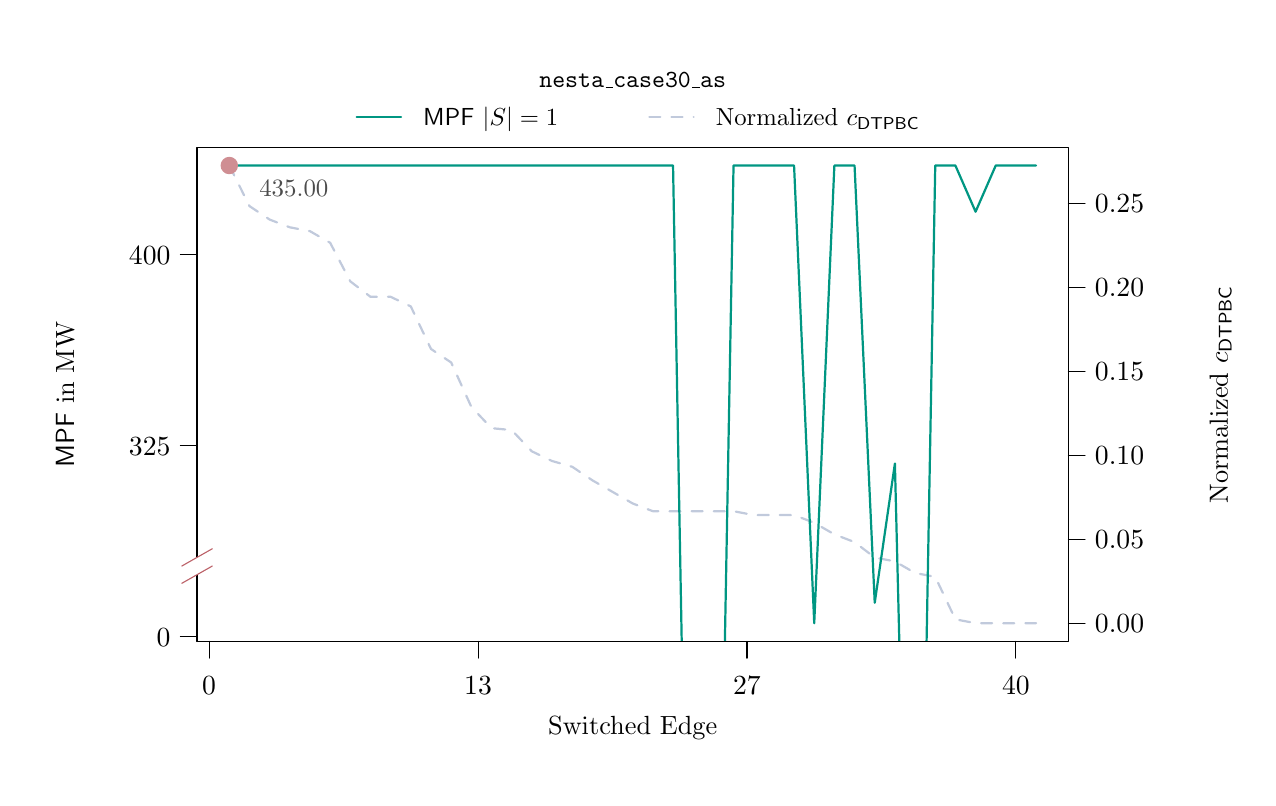
\begin{tikzpicture}[x=1pt,y=1pt]
\definecolor{fillColor}{RGB}{255,255,255}
\path[use as bounding box,fill=fillColor,fill opacity=0.00] (0,0) rectangle (440.85,271.01);
\begin{scope}
\path[clip] (  0.00,  0.00) rectangle (440.85,271.01);
\definecolor{drawColor}{RGB}{193,202,220}

\path[draw=drawColor,line width= 0.8pt,dash pattern=on 4pt off 4pt ,line join=round,line cap=round] ( 72.86,221.20) --
	( 80.15,206.54) --
	( 87.44,201.66) --
	( 94.73,198.87) --
	(102.01,197.47) --
	(109.30,193.28) --
	(116.59,179.33) --
	(123.88,173.75) --
	(131.17,173.75) --
	(138.45,170.26) --
	(145.74,154.90) --
	(153.03,150.02) --
	(160.32,133.97) --
	(167.61,126.29) --
	(174.89,125.60) --
	(182.18,117.92) --
	(189.47,114.43) --
	(196.76,112.34) --
	(204.05,107.45) --
	(211.34,103.27) --
	(218.62, 99.08) --
	(225.91, 96.29) --
	(233.20, 96.29) --
	(240.49, 96.29) --
	(247.78, 96.29) --
	(255.06, 96.29) --
	(262.35, 94.89) --
	(269.64, 94.89) --
	(276.93, 94.89) --
	(284.22, 92.10) --
	(291.50, 87.91) --
	(298.79, 85.12) --
	(306.08, 79.54) --
	(313.37, 78.15) --
	(320.66, 73.96) --
	(327.95, 72.56) --
	(335.23, 57.21) --
	(342.52, 55.82) --
	(349.81, 55.82) --
	(357.10, 55.82) --
	(364.39, 55.82);
\end{scope}
\begin{scope}
\path[clip] (  0.00,  0.00) rectangle (440.85,271.01);
\definecolor{drawColor}{RGB}{0,0,0}

\path[draw=drawColor,line width= 0.4pt,line join=round,line cap=round] ( 61.20, 49.20) --
	(376.05, 49.20) --
	(376.05,227.81) --
	( 61.20,227.81) --
	( 61.20, 49.20);
\end{scope}
\begin{scope}
\path[clip] (  0.00,  0.00) rectangle (440.85,271.01);
\definecolor{drawColor}{RGB}{0,0,0}

\path[draw=drawColor,line width= 0.4pt,line join=round,line cap=round] (376.05, 55.82) -- (376.05,207.59);

\path[draw=drawColor,line width= 0.4pt,line join=round,line cap=round] (376.05, 55.82) -- (382.05, 55.82);

\path[draw=drawColor,line width= 0.4pt,line join=round,line cap=round] (376.05, 86.17) -- (382.05, 86.17);

\path[draw=drawColor,line width= 0.4pt,line join=round,line cap=round] (376.05,116.53) -- (382.05,116.53);

\path[draw=drawColor,line width= 0.4pt,line join=round,line cap=round] (376.05,146.88) -- (382.05,146.88);

\path[draw=drawColor,line width= 0.4pt,line join=round,line cap=round] (376.05,177.23) -- (382.05,177.23);

\path[draw=drawColor,line width= 0.4pt,line join=round,line cap=round] (376.05,207.59) -- (382.05,207.59);

\node[text=drawColor,anchor=base west,inner sep=0pt, outer sep=0pt, scale=  1.00] at (385.65, 52.37) {0.00};

\node[text=drawColor,anchor=base west,inner sep=0pt, outer sep=0pt, scale=  1.00] at (385.65, 82.73) {0.05};

\node[text=drawColor,anchor=base west,inner sep=0pt, outer sep=0pt, scale=  1.00] at (385.65,113.08) {0.10};

\node[text=drawColor,anchor=base west,inner sep=0pt, outer sep=0pt, scale=  1.00] at (385.65,143.44) {0.15};

\node[text=drawColor,anchor=base west,inner sep=0pt, outer sep=0pt, scale=  1.00] at (385.65,173.79) {0.20};

\node[text=drawColor,anchor=base west,inner sep=0pt, outer sep=0pt, scale=  1.00] at (385.65,204.15) {0.25};
\end{scope}
\begin{scope}
\path[clip] (  0.00,  0.00) rectangle (440.85,271.01);
\definecolor{drawColor}{RGB}{0,150,130}

\path[draw=drawColor,line width= 0.8pt,line join=round,line cap=round] (118.89,238.60) -- (134.91,238.60);
\definecolor{drawColor}{RGB}{193,202,220}

\path[draw=drawColor,line width= 0.8pt,dash pattern=on 4pt off 4pt ,line join=round,line cap=round] (224.63,238.60) -- (240.65,238.60);
\definecolor{drawColor}{RGB}{0,0,0}

\node[text=drawColor,anchor=base,inner sep=0pt, outer sep=0pt, scale=  0.89] at (218.62,249.28) {\texttt{nesta\_case30\_as}};

\node[text=drawColor,anchor=base west,inner sep=0pt, outer sep=0pt, scale=  0.89] at (142.92,235.54) {$\mathsf{MPF}~|S|=1$};

\node[text=drawColor,anchor=base west,inner sep=0pt, outer sep=0pt, scale=  0.89] at (248.66,235.54) {Normalized~$c_\mathsf{DTPBC}$};
\end{scope}
\begin{scope}
\path[clip] (  0.00,  0.00) rectangle (440.85,271.01);
\definecolor{drawColor}{RGB}{0,0,0}

\path[draw=drawColor,line width= 0.4pt,line join=round,line cap=round] ( 61.20, 50.90) -- ( 61.20,188.98);

\path[draw=drawColor,line width= 0.4pt,line join=round,line cap=round] ( 61.20, 50.90) -- ( 55.20, 50.90);

\path[draw=drawColor,line width= 0.4pt,line join=round,line cap=round] ( 61.20,119.94) -- ( 55.20,119.94);

\path[draw=drawColor,line width= 0.4pt,line join=round,line cap=round] ( 61.20,188.98) -- ( 55.20,188.98);

\node[text=drawColor,anchor=base east,inner sep=0pt, outer sep=0pt, scale=  1.00] at ( 51.60, 47.45) {0};

\node[text=drawColor,anchor=base east,inner sep=0pt, outer sep=0pt, scale=  1.00] at ( 51.60,116.49) {325};

\node[text=drawColor,anchor=base east,inner sep=0pt, outer sep=0pt, scale=  1.00] at ( 51.60,185.53) {400};
\end{scope}
\begin{scope}
\path[clip] (  0.00,  0.00) rectangle (440.85,271.01);
\definecolor{drawColor}{RGB}{255,255,255}
\definecolor{fillColor}{RGB}{255,255,255}

\path[draw=drawColor,line width= 0.4pt,line join=round,line cap=round,fill=fillColor] ( 55.69, 73.34) rectangle ( 66.71, 79.59);
\definecolor{drawColor}{RGB}{188,97,104}

\path[draw=drawColor,line width= 0.4pt,line join=round,line cap=round] ( 55.69, 70.22) -- ( 66.71, 76.47);

\path[draw=drawColor,line width= 0.4pt,line join=round,line cap=round] ( 55.69, 76.47) -- ( 66.71, 82.72);
\end{scope}
\begin{scope}
\path[clip] ( 61.20, 49.20) rectangle (376.05,227.81);
\definecolor{drawColor}{RGB}{0,150,130}

\path[draw=drawColor,line width= 0.8pt,line join=round,line cap=round] ( 72.86,221.20) --
	( 80.15,221.20) --
	( 87.44,221.20) --
	( 94.73,221.20) --
	(102.01,221.20) --
	(109.30,221.20) --
	(116.59,221.20) --
	(123.88,221.20) --
	(131.17,221.20) --
	(138.45,221.20) --
	(145.74,221.20) --
	(153.03,221.20) --
	(160.32,221.20) --
	(167.61,221.20) --
	(174.89,221.20) --
	(182.18,221.20) --
	(189.47,221.20) --
	(196.76,221.20) --
	(204.05,221.20) --
	(211.34,221.20) --
	(218.62,221.20) --
	(225.91,221.20) --
	(233.20,221.20) --
	(237.23,  0.00);

\path[draw=drawColor,line width= 0.8pt,line join=round,line cap=round] (251.04,  0.00) --
	(255.06,221.20) --
	(262.35,221.20) --
	(269.64,221.20) --
	(276.93,221.20) --
	(284.22, 55.82) --
	(291.50,221.20) --
	(298.79,221.20) --
	(306.08, 63.18) --
	(313.37,113.51) --
	(316.19,  0.00);

\path[draw=drawColor,line width= 0.8pt,line join=round,line cap=round] (323.92,  0.00) --
	(327.95,221.20) --
	(335.23,221.20) --
	(342.52,204.50) --
	(349.81,221.20) --
	(357.10,221.20) --
	(364.39,221.20);
\end{scope}
\begin{scope}
\path[clip] ( 61.20, 49.20) rectangle (376.05,227.81);
\definecolor{fillColor}{RGB}{207,142,147}

\path[fill=fillColor] ( 72.86,221.20) circle (  3.15);
\end{scope}
\begin{scope}
\path[clip] ( 61.20, 49.20) rectangle (376.05,227.81);
\definecolor{drawColor}{gray}{0.30}

\node[text=drawColor,anchor=base,inner sep=0pt, outer sep=0pt, scale=  0.90] at ( 96.18,210.04) {435.00};
\end{scope}
\begin{scope}
\path[clip] (  0.00,  0.00) rectangle (440.85,271.01);
\definecolor{drawColor}{RGB}{0,0,0}

\path[draw=drawColor,line width= 0.4pt,line join=round,line cap=round] ( 65.57, 49.20) -- (357.10, 49.20);

\path[draw=drawColor,line width= 0.4pt,line join=round,line cap=round] ( 65.57, 49.20) -- ( 65.57, 43.20);

\path[draw=drawColor,line width= 0.4pt,line join=round,line cap=round] (162.75, 49.20) -- (162.75, 43.20);

\path[draw=drawColor,line width= 0.4pt,line join=round,line cap=round] (259.92, 49.20) -- (259.92, 43.20);

\path[draw=drawColor,line width= 0.4pt,line join=round,line cap=round] (357.10, 49.20) -- (357.10, 43.20);

\node[text=drawColor,anchor=base,inner sep=0pt, outer sep=0pt, scale=  1.00] at ( 65.57, 30.00) {0};

\node[text=drawColor,anchor=base,inner sep=0pt, outer sep=0pt, scale=  1.00] at (162.75, 30.00) {13};

\node[text=drawColor,anchor=base,inner sep=0pt, outer sep=0pt, scale=  1.00] at (259.92, 30.00) {27};

\node[text=drawColor,anchor=base,inner sep=0pt, outer sep=0pt, scale=  1.00] at (357.10, 30.00) {40};

\node[text=drawColor,anchor=base,inner sep=0pt, outer sep=0pt, scale=  0.95] at (218.62, 15.60) {Switched Edge};

\node[text=drawColor,rotate= 90.00,anchor=base,inner sep=0pt, outer sep=0pt, scale=  0.95] at ( 16.80,138.51) {$\mathsf{MPF}$ in~$\mathrm{MW}$};

\node[text=drawColor,rotate= 90.00,anchor=base,inner sep=0pt, outer sep=0pt, scale=  0.95] at (433.65,138.51) {Normalized~$c_\mathsf{DTPBC}$};
\end{scope}
\end{tikzpicture}
